\section{Results and Discussion}
\label{sec:results}

\subsection{Main Results}

Table~\ref{tab:main_results} reports the performance of all four methods on each dataset. We present all seven metrics for completeness; the primary metric for comparison is Recall@K, which captures ranking quality at the operational threshold where a fixed number of top-scoring nodes would be investigated.

\begin{table}[h]
\centering
\caption{Main results across four datasets. Best per metric in bold.}
\label{tab:main_results}
\resizebox{\textwidth}{!}{%
\begin{tabular}{llccccccc}
\toprule
Dataset & Method & AUC & AP & MF1 & Recall & Prec & Recall@K & Acc \\
\midrule
\multirow{4}{*}{YelpChi} 
& GAAP      & 0.9866 & 0.9468 & 0.9292 & 0.8339 & \textbf{0.9257} & 0.8839 & 0.9667 \\
& +Focal    & 0.9859 & \textbf{0.9524} & 0.9314 & 0.8769 & 0.8872 & 0.8839 & 0.9666 \\
& RP-GAAP   & \textbf{0.9867} & 0.9515 & \textbf{0.9344} & \textbf{0.8839} & 0.8907 & \textbf{0.8885} & \textbf{0.9688} \\
& +Focal     & 0.9827 & 0.9321 & 0.9176 & 0.8077 & 0.9130 & 0.8700 & 0.9608 \\
\midrule
\multirow{4}{*}{T-Finance} 
& GAAP      & 0.9672 & 0.9046 & 0.9219 & 0.8142 & 0.8907 & 0.8488 & 0.9870 \\
& +Focal    & 0.9706 & 0.9000 & 0.9290 & 0.8155 & 0.9188 & 0.8571 & 0.9726 \\
& RP-GAAP   & 0.9715 & 0.8981 & \textbf{0.9370} & 0.8239 & \textbf{0.9429} & \textbf{0.8599} & 0.9870 \\
& +Focal     & \textbf{0.9741} & \textbf{0.9079} & 0.9314 & \textbf{0.8363} & 0.9041 & 0.8571 & \textbf{0.9882} \\
\midrule
\multirow{4}{*}{Elliptic} 
& GAAP      & 0.9257 & 0.7908 & 0.8737 & 0.7285 & 0.8010 & 0.7322 & 0.9697 \\
& +Focal    & 0.9343 & 0.7962 & 0.8712 & \textbf{0.7295} & 0.7900 & \textbf{0.7359} & \textbf{0.9734} \\
& RP-GAAP   & \textbf{0.9377} & \textbf{0.8016} & \textbf{0.8869} & 0.7193 & \textbf{0.8694} & \textbf{0.7359} & 0.9656 \\
& +Focal     & 0.9310 & 0.7936 & 0.8638 & 0.7267 & 0.7641 & 0.7322 & 0.9479 \\
\midrule
\multirow{4}{*}{Tolokers} 
& GAAP      & 0.8419 & 0.5661 & 0.7084 & 0.5358 & \textbf{0.5495} & 0.5498 & \textbf{0.8095} \\
& +Focal    & 0.8440 & \textbf{0.5776} & 0.7147 & 0.6511 & 0.5091 & 0.5561 & 0.7381 \\
& RP-GAAP   & \textbf{0.8460} & 0.5765 & \textbf{0.7288} & 0.6386 & 0.5423 & \textbf{0.5623} & 0.8085 \\
& +Focal     & 0.8380 & 0.5716 & 0.7116 & \textbf{0.6573} & 0.5012 & \textbf{0.5623} & 0.7568 \\
\bottomrule
\end{tabular}%
}
\end{table}

\paragraph{Recall@K analysis.}
Table~\ref{tab:recall_at_k} extracts the primary metric for direct comparison across methods and datasets. RP-GAAP achieves the best Recall@K on YelpChi~(+0.46) and T-Finance~(+1.11), while the combined RP-GAAP+Focal ties for best on Elliptic~(+0.37) and ties with RP-GAAP on Tolokers~(+1.25). The largest absolute gain is observed on Tolokers, where RP-GAAP and the combined variant both achieve 0.5623 vs.\ the baseline 0.5498. On Elliptic, RP-GAAP and focal loss both reach 0.7359, offering a modest improvement over the 0.7322 baseline.

\begin{table}[h]
\centering
\caption{Recall@K scores (primary metric) across datasets and methods. Best per dataset in bold. $\Delta$ is the absolute gain of the best method over GAAP, scaled $\times 10^2$.}
\label{tab:recall_at_k}
\begin{tabular}{lcccc|c}
\toprule
Dataset & GAAP & +Focal & RP-GAAP & +Focal & Best $\Delta$ \\
\midrule
YelpChi     & 0.8839 & 0.8839 & \textbf{0.8885} & 0.8700 & +0.46 (Rare) \\
T-Finance   & 0.8488 & 0.8571 & \textbf{0.8599} & 0.8571 & \textbf{+1.11} (Rare) \\
Elliptic    & 0.7322 & \textbf{0.7359} & \textbf{0.7359} & 0.7322 & +0.37 (Rare/Focal) \\
Tolokers    & 0.5498 & 0.5561 & \textbf{0.5623} & \textbf{0.5623} & +1.25 (Rare/Both) \\
\bottomrule
\end{tabular}
\end{table}

\subsection{Discussion}

Several patterns emerge from the main results. First, rare-pattern weighting alone tends to dominate on datasets where GAAP already performs well (YelpChi, T-Finance), while the combination with focal loss proves more competitive on harder benchmarks (Tolokers). This suggests that rarity-based weighting improves discrimination when the model can already rank most nodes correctly, and difficulty-based focal loss provides complementary benefit when classification confidence is genuinely low. Second, the precision-recall tradeoff holds consistently: where recall improves, precision tends to drop, though RP-GAAP maintains higher precision than focal loss on YelpChi (0.8907 vs.\ 0.8872). Third, Elliptic is partially responsive to loss-level interventions---RP-GAAP and focal loss both reach 0.7359 Recall@K, a modest improvement over the 0.7322 baseline---but the gains remain smaller than on the other datasets, consistent with its temporal graph structure where static feature binning may produce a sparse pattern space.

\subsection{Hyperparameter Sensitivity}

To understand the sensitivity of RP-GAAP to its four hyperparameters, we ran a grid sweep on Tolokers, varying one parameter at a time around the default settings. Tolokers was chosen because it shows the largest performance gap and the most room for improvement. Table~\ref{tab:sweep} summarizes the best Recall@K achieved by sweeping each parameter individually.

\begin{table}[h]
\centering
\caption{Hyperparameter sweep on Tolokers (28 runs). Gain is the Recall@K difference between the best value and the default, scaled $\times 10^2$.}
\label{tab:sweep}
\begin{tabular}{lcccc}
\toprule
Parameter & Default & Swept Values & Best & Gain \\
\midrule
rare\_num\_bins      & 5   & \{3, 5, 7\}        & 7    & +1.39 \\
rare\_top\_k\_features & 10  & \{5, 10, 15\}      & 5    & +1.56 \\
rare\_max\_weight     & 3.0 & \{1.5, 2.0, 3.0, 5.0\} & 5.0  & +1.56 \\
rare\_fraud\_boost    & 1.5 & \{1.0, 1.5, 2.0, 3.0\} & 1.0  & +1.39 \\
focal\_alpha (class 1) & 3.0 & \{1.5, 2.0, 3.0, 4.0\} & 2.0  & +0.29 \\
\bottomrule
\end{tabular}
\end{table}

The sweep reveals that the default hyperparameters are conservative: reducing $k$ from 10 to 5 features and increasing $w_{\text{max}}$ from 3.0 to 5.0 each provide a Recall@K gain of roughly 1.5 points over the default RP-GAAP configuration. However, the Recall@K noise floor on Tolokers is estimated at approximately $\pm$0.02 based on the observed variance across the sweep runs, so individual gains below roughly 2 points should be interpreted cautiously. The key insight is that the method is not brittle: all swept values produce performance within a narrow band, and no parameter setting causes catastrophic degradation.

Figure~\ref{fig:sweep} visualizes the sweep results across all five parameters.

\begin{figure}[h]
\centering
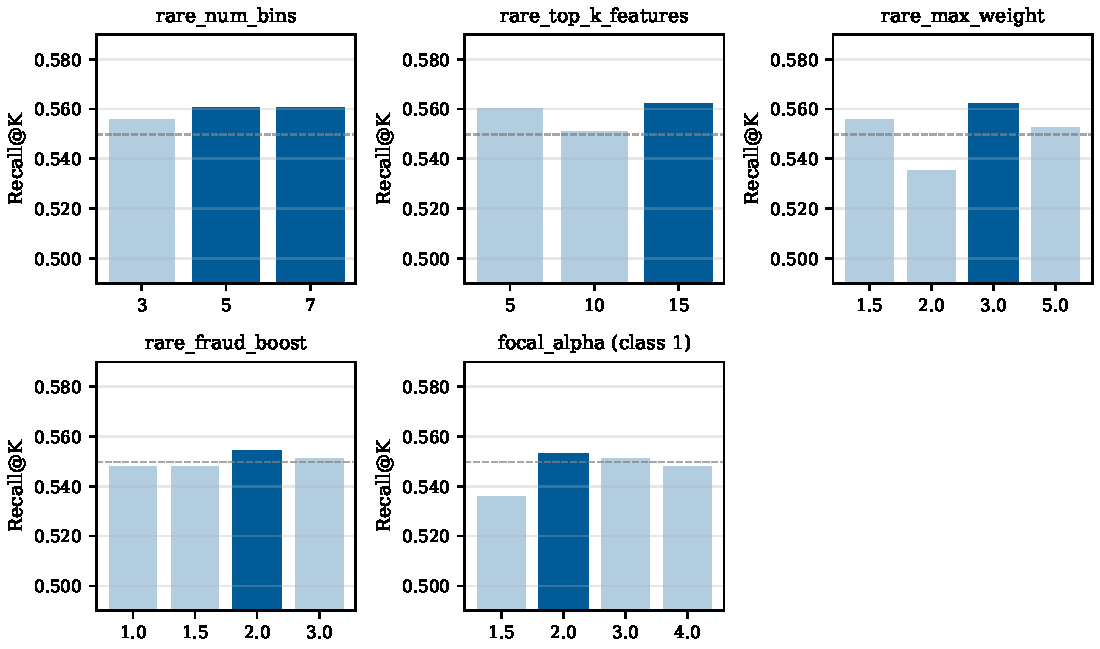
\includegraphics[width=\textwidth]{Figures/sweep_tolokers.pdf}
\caption{Hyperparameter sensitivity on Tolokers. Each subplot shows Recall@K as a function of a single parameter, with all others held at default values. The dashed horizontal line indicates the GAAP baseline Recall@K.}
\label{fig:sweep}
\end{figure}
